\documentclass[../main.tex]{subfiles}


\begin{document}
\raggedright
Data will eventually need to be stored in a database and to do a schema for a database must exist. Figure \ref{fig:dbschema} shows the final schema currently implemented. This schema was updated twice based on Django migration logs. All-Auth\cite{allauth} automatically generated \textit{Authuser} and the rest of the tables are designed specifically to the requirements. All the fields were designed before implementation except for \textit{userlink} in the \textit{userprofile} table and \textit{moreproof} in the \textit{ecfdata} table. These were added during implementation to allow the students to have a unique public data and to allow the additional proof to be uploaded with the use of notifications respectively. The tables are interlinked between each other; The \textit{user} table has a one to many relationship with \textit{ecfdata} and a one to one relation with \textit{userprofile} and \textit{publicecf}. Along with the user table, the \textit{ecfdata} table is linked with a one to many relationship to both \textit{moduledata} and \textit{files}. These simple relationships make it easy to input data into them without having issues when running queries. 

\begin{figure}[H]
        \begin{center}
        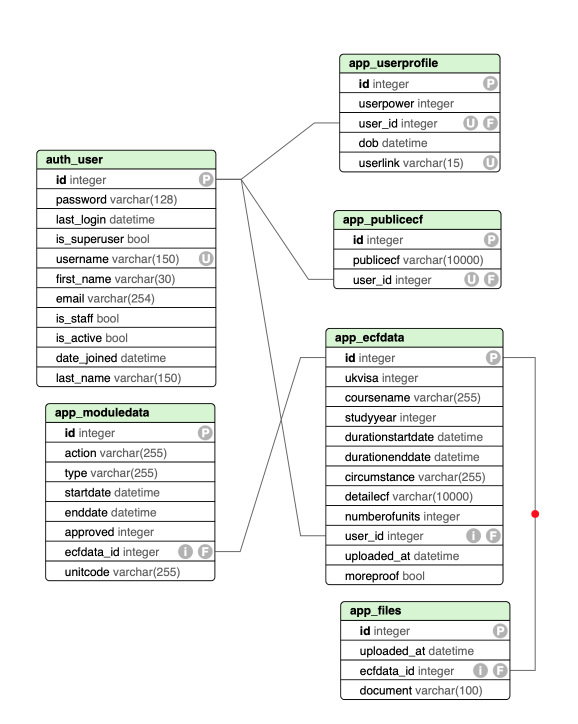
\includegraphics[scale=1.2]
        {images/db.png}
        \caption{\label{fig:dbschema} Database Schema}
        \end{center}
      \end{figure}
  
  
\end{document}
